Matlabbs huvudsyfte är att låta användaren spara information om recept
och råvaror i en databas och erbjuder en uppsättning funktioner för
att lägga till, ändra, söka efter och läsa recept.

De funktioner som finns tillgängliga är:
\begin{itemize}
\item Läsa recept
\item Söka efter recept
\item Lägga till/redigera recept
\item Lägga till/redigera ingredienser
\item Import/export via .xml samt export till .txt
\end{itemize}

För att göra detta möjligt används ett grafiskt gränssnitt som de
flesta användare säkert redan känner sig bekanta med. Gränssnittet
består av ett stort huvudfönster med flikar som skickar dig mellan de
olika vyerna. I figur \ref{fig:oversikt} finns en överblicksbild som
visar gränssnittet.

\begin{figure}[H]
        \centering 
        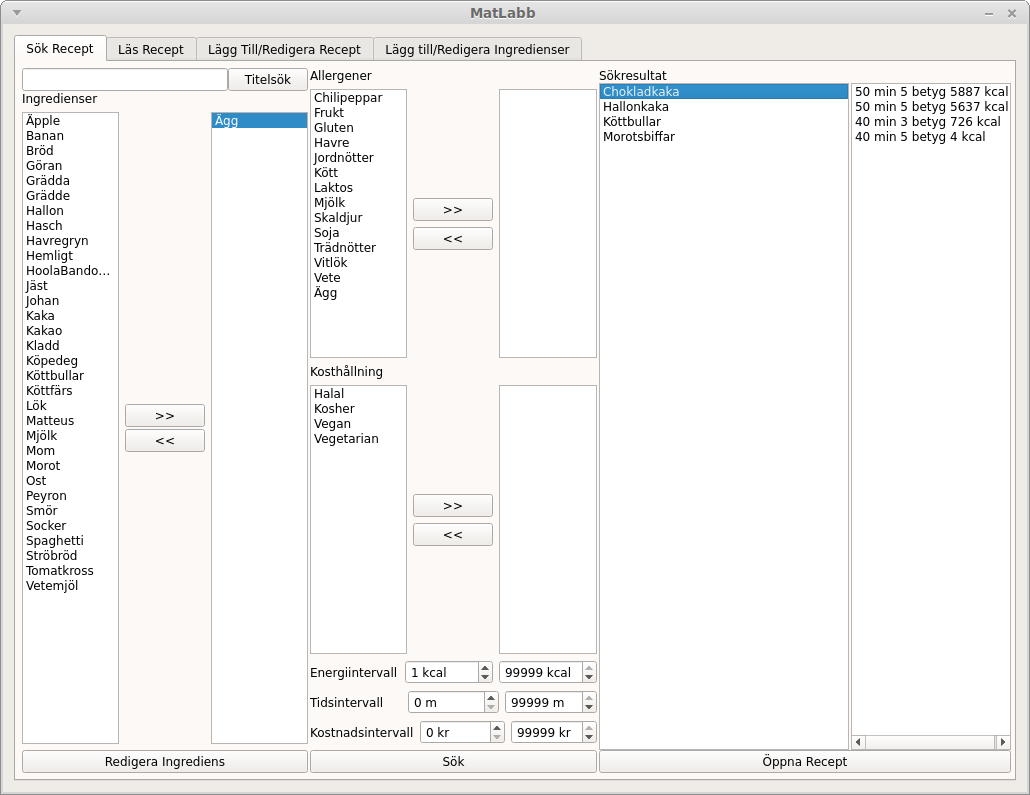
\includegraphics[scale=0.40]{sok_recept.png} 
        \caption{Sökvyn} 
        \label{fig:oversikt}
\end{figure}

Matlabb styrs nästan uteslutande med hjälp av musen och för att
använda olika funktioner eller växla vy används räcker det att klicka
på rätt knapp. När recept eller ingredienser redigeras kan text matas
in med hjälp av tangentbordet i motsvarande textruta.


